
\documentclass{standalone}

%\documentclass[convert]{standalone}
% convert: in addition to pdf output files, png files are created
% convert options does work properly with -output-directory option of latexmk

\usepackage{tikz-feynman}
\tikzfeynmanset{compat=1.1.0}


\begin{document}
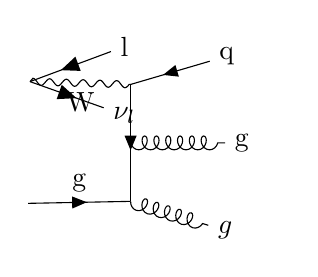
\begin{tikzpicture}
          \begin{feynman}
            \diagram [small, vertical=a to b] {
            % t-channel ttbar, qq -> gg -- > bbtt

            qi1 [particle=q] -- [fermion] a -- [boson, edge label=W] w1,
            qo2 -- [fermion, edge label=g] b -- [gluon] gi2 [particle=\( g \)] ,

            a -- [fermion] b,

            % invisible helper
            qi1 -- [draw=none] invis -- [draw=none] gi2,
            w1 -- [draw=none] qo2,
            };

            % w1 decay
            \vertex [right=1.2cm of w1] (b12_invis_helper);    % helper
            \vertex [above=0.2cm of b12_invis_helper] (b1) {l};
            \vertex [below=0.2cm of b12_invis_helper] (b2) {$\nu_{l}$};
            \draw [fermion] (b1) -- (w1);
            \draw [fermion] (w1) -- (b2);

            % qo2 decay
            % \vertex [right=1.2cm of qo2] (t12_invis_helper);    % helper
            % \vertex [above=0.2cm of t12_invis_helper] (qo1) {q};
            % \vertex [below=0.2cm of t12_invis_helper] (qo2) {q};
            % \draw [fermion] (qo1) -- (qo2);
            % \draw [fermion] (qo2) -- (qo2);

            % radiation from virtual t-channel particle
            \vertex at ($(a)!0.5!(b)$) (r_start);
            \vertex [right=1.2cm of r_start] (r_end) {g};
            \draw [gluon] (r_start) -- (r_end);

          \end{feynman}
        \end{tikzpicture}
\end{document}
